\graphicspath{{./chapters/chapter08/}}
\chapter{Линейная модель}

\begin{exmp}[\textbf{Линейная регрессия}]
	Предположим, что $X$ и $Y$ связаны следующим соотношением:
	\[ Y = b_0 + b_1 X, \]
	и мы хотим оценить значения $b_0$ и $b_1$. На практике рассматривается не строгая линейная зависимость, а соотношение вида
	\[ Y_i = b_0 + b_1 X_i + \varepsilon_i \quad \forall i = 1, \dots, n, \]
	где $\varepsilon_i$ -- ошибка, такая что $\ME[\varepsilon_i] = 0$ и $\Var(\varepsilon_i) = \sigma^2 > 0$. В векторной записи: $Y = Xb + \varepsilon$ или
	\[  \begin{pmatrix}
	Y_1 \\
	\vdots \\
	Y_n
	\end{pmatrix}  = 
	\begin{pmatrix}
	1 & X_1 \\
	\vdots & \vdots \\
	1 & X_n
	\end{pmatrix}
	\begin{pmatrix}
	b_0 \\
	b_1
	\end{pmatrix}
	+
	\begin{pmatrix}
	\varepsilon_1 \\
	\vdots \\
	\varepsilon_n
	\end{pmatrix}.\] 
\end{exmp}

\begin{exmp}[\textbf{Анализ дисперсии}]
	Рассмотрим эксперимент: разделим $n$ животных на $a$ групп по типу питания. В каждой $i$-й группе $n_i$ животных. Смоделируем вес каждого животного:
	\[ Y_{ij} = \mu_i + \varepsilon_{ij}, \quad i = 1, \dots, a,\ j = 1, \dots, n_i. \]
	В векторной записи: $Y = X\mu + \varepsilon$ или
	\[ \begin{pmatrix}
	Y_{11} \\
	\vdots \\
	Y_{1n_1} \\
	\vdots \\
	Y_{a1} \\
	\vdots \\
	Y_{an_a}
	\end{pmatrix}  =
	\begin{pmatrix}
	\mathds{1}_{n_1} & 0 & \dots & 0\\
	0 & \mathds{1}_{n_2} & \dots & 0 \\
	\vdots & \vdots & \vdots & \vdots \\
	0 & 0 & \dots & \mathds{1}_{n_a}
	\end{pmatrix}
	\begin{pmatrix}
	\mu_{1} \\
	\vdots \\
	\mu_{a}
	\end{pmatrix} +
	\begin{pmatrix}
	\varepsilon_{11} \\
	\vdots \\
	\varepsilon_{1n_1} \\
	\vdots \\
	\varepsilon_{a1} \\
	\vdots \\
	\varepsilon_{an_a}
	\end{pmatrix}
	\]
	Вопрос: как оценить $\mu_i$ и протестировать $\mu_1 = \dots = \mu_a$?
\end{exmp}

\begin{defn}
	Пусть $X \in \MR^{n \times k}$ и $b \in \MR^k$, $n > k$ и пусть $\varepsilon = (\varepsilon_1, \dots, \varepsilon_n)^T$ -- $n$-мерный случайный вектор.
	\begin{enumerate}
		\item Если $\varepsilon \sim \mathcal{N}_n(0, \sigma^2 \mathds{1}_n)$, то $Y = Xb + \varepsilon$ называется \textbf{\textit{линейной моделью с предположением нормальности (LMN)}}.
		\item Пусть $Z \sim \mathcal{N}(0, \sigma^2 \mathds{1}_n)$. Если
		\[ \ME[\varepsilon_{i_1}\varepsilon_{i_2}\varepsilon_{i_3}\varepsilon_{i_4}]  = \ME[Z_{i_1}Z_{i_2}Z_{i_3}Z_{i_4}] \quad \forall i_j \in \{ 1, \dots, n \}, \]
		то $Y = Xb + \varepsilon$ называется \textbf{\textit{линейной моделью с предположением о моментах (LMM)}}.
		\item $X$ называется \textbf{\textit{матрицей плана}}.
	\end{enumerate}
\end{defn}

\begin{rmrk}
	Если ранг матрицы $X$ равен $r$ и
	\begin{center}\centering
		\begin{minipage}{0.18\linewidth}
				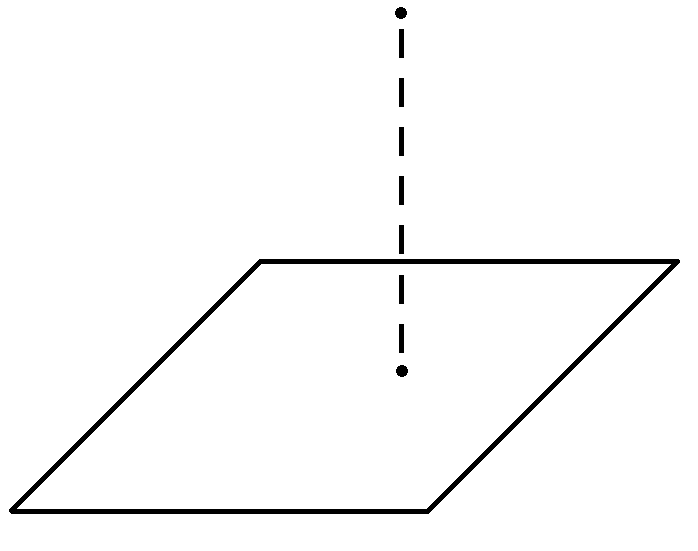
\includegraphics[width=\linewidth, height=2.0cm, right]{projection}
				\captionsetup{labelformat=empty}
				\put(-37, 60){$Y$}
				\put(-53, 40){\large $\searrow$}
				\put(-63, 50){$P$}
				\put(-35, 17){$X\hat b$}
				\put(-100, 20){$R(X)$}
		\end{minipage}
		\begin{minipage}{0.7\textwidth}
			\[R(X) = \{Xb\ | \ b \in \MR^k \} \in \MR^n \]
			её диапазон, то наивной оценкой $Xb$ является ортогональная проекция $Y$ на $R(X)$. Тогда любой вектор $\hat b$ такой, что $P(Y) = X \hat b$ является приемлемой оценкой $b$.
		\end{minipage}
	\end{center}	
\end{rmrk}

\begin{defn}
	Мы назовем $G \in \MR^{n \times m}$ \textbf{\textit{обобщенной обратной матрицей}} к матрице $A \in \MR^{m \times n}$, если
	\[ AGA = A. \]
	Зададим множество обобщенных обратных к $A$ матриц:
	\[ A^- = \{ G \ |\ AGA = A \}. \]
\end{defn}

\begin{rmrk}
	Мы будем писать $A^-$ вместо $G$, если действенность формулы не зависит то выбора обобщенной обратной матрицы. Например, $AA^-A=A$.
\end{rmrk}

\begin{exmp}
	Пусть 
	\[ A = \begin{pmatrix}
	1 & 1 \\
	1 & 1
	\end{pmatrix}. \]
	Обобщенные обратные матрицы, например:
	\[ 
	G_1 = \frac{1}{4}
	\begin{pmatrix}
	 1 & 1 \\
	 1 & 1
	\end{pmatrix}
	\quad \text{и} \quad
	G_2 = \frac{1}{2}
	\begin{pmatrix}
	1 & 0 \\
	0 & 1
	\end{pmatrix}.
	\]
\end{exmp}

\begin{lmm}[\textbf{Включение диапазона}] \label{Range inclusion}
	Пусть $X \in \MR^{n \times k}$ и $V \in \MR^{n \times s}$. Тогда:
	\begin{enumerate}
		\item $R(X) \subset R(V) \quad \Longleftrightarrow \quad VV^-X = X.$
		\item Если (i) соблюдается и $V \geq 0$ (также $n = s$), то
		\begin{enumerate}
			\item $X^T V^-X = 0,$
			\item $R(X^T) = R(X^TV^-X).$
		\end{enumerate}
	\end{enumerate}
\end{lmm}
\begin{proof}
	\begin{enumerate}
		\item Напомним, что
		\[ R(X) \subset R(V) \quad \Longleftrightarrow \quad X = VW. \]
		
		''$\Longleftarrow$'' \checkmark. \\
		''$\Longrightarrow$'' Пусть $X = VW$ и $G$ -- обобщенная обратная матрица $V$. Тогда
		\[ VGX = VGVW = VW = X. \]
		\item
		\begin{enumerate}
			\item Пусть $G$ -- обобщенная обратная матрица $V$. Тогда вследствие симметричности $V$
		    \[ X^TGX = W^TV^TGVW = W^TVW \geq 0. \]
		    \item Напомним некоторые теоремы из линейной алгебры:
		    \begin{enumerate}
		    	\item Матрица $V$ симметричная и положительно полуопределенная $\Longrightarrow$ её собственные числа $\lambda_i$ вещественные и неотрицательные
		    	$\Longrightarrow V = \sum_{i=1}^n \lambda_i z_i z_i^T$ ($z_i$ -- ортонормальные собственные вектора)
		    	$\Longrightarrow V^\alpha = \sum_{i=1}^{n} \lambda_i^\alpha z_i z_i^T$ для $\alpha \geq 0$ и $V^{\alpha + \beta} = V^\alpha V^\beta$.
		    	\item $r(A) = r(A^TA)$ и $r(A \cdot B) \leq \min{\{r(A), r(B)\}}$.
		    	В частности, $r(VW) = r(W^TVW)$, так как
		    	\[ r(VW) = r(V^{\frac{1}{2}}V^{\frac{1}{2}}W) \leq r(V^{\frac{1}{2}}W) = r(W^TVW) \leq \min \{r(W^T), r(VW) \}.   \]
		    	Используя (a), мы получаем:
		    	\[ r(X^TV^-X) = r(W^TVW) = r(VW) = r(VV^-X) = r(X). \]
		    \end{enumerate}
    	\end{enumerate}  
	\end{enumerate}
\end{proof}

\begin{thm}
	В линейной модели $Y = Xb + \varepsilon$ ортогональная проекция $Y$ на $R(X)$ и её ортогональное дополнение
	\[ R(X)^{\perp} = \{Z\ | \ Z^TX = 0 \}  \]
	задаются как
	\[P = X(X^T X)^- X^T \quad \text{и} \quad R = \mathbb{I}_n - P \]
	соответственно.
\end{thm}
\begin{proof}
	Мы докажем только для $P$. Для ортогональной проекции имеют место равенства $P^T = P$ и $P^2=P$. Во-первых,
	\[ (X^TX)(X^TX)^-X^T = VV^-X^T = X^T \]
	по Лемме \ref{Range inclusion}(i) и (ii)(b). Тогда
	\[ P^2 = X(X^TX)^-X^TX(X^TX)^-X^T = X(X^TX)^-X^T = P\]
	и $P^T = P$ следует из Леммы \ref{Range inclusion} (ii)(a).
	Наконец, $P(Y) \in R(X)$, так как $P$ вида $XA$, где $A = (X^TX)^-X^T$. Также,
	\[ P(Xb) = X(X^TX)^-X^TXb = Xb. \]
\end{proof}

\begin{rmrk} \label{rmrk8.10} \
	\begin{enumerate}
		\item Разумными оценками для $Xb$ и $\sigma^2$ являются
		\[ X\hat{b} = P(Y) = X(X^TX)^-X^TY  \]
		и
		\[ \hat{\sigma}^2 = \frac{\| Y - X\hat{b} \|_2^2}{n - r} = \frac{\| RY \|_2^2}{n - r} = \frac{Y^TRY}{n - r}, \]
		где выбор знаменателя $n-r$ будет обоснован в Следствии \ref{crlr8.13}.
		\item В общем случае, не существует единственной оценки для $b$. Однако если матрица $X^TX$ обратима ($r=r(X)=k$), то
		\[X^TX\hat{b} = X^TX(X^TX)^{-1}X^TY=X^TY  \]
		и
		\[ \hat{b} = (X^TX)^{-1}X^TY. \]
		Заметим также, что
		\[ \ME[\hat{b}] = (X^TX)^{-1}X^T\ME[Y] = (X^TX)^{-1}X^TXb = b. \]
	\end{enumerate}
\end{rmrk}

\begin{exmp}
	Пусть $Y_1, \dots, Y_n$ i.i.d. $\sim \mathcal{N}(\mu, \sigma^2)$, такие что:
	\[ Y = \begin{pmatrix}
	Y_1 \\
	\vdots \\
	Y_n
	\end{pmatrix}
	=
	 \begin{pmatrix}
	 1 \\
	 \vdots \\
	 1
	 \end{pmatrix}
	 \mu +
	  \begin{pmatrix}
	  \varepsilon_1 \\
	  \vdots \\
	  \varepsilon_n
	  \end{pmatrix}
	  = X \mu + \varepsilon,
	  	 \]
	 где $\varepsilon_1, \dots, \varepsilon_n$ i.i.d. $\sim \mathcal{N}(0, \sigma^2)$. Так как
	 \[ X^TX = (1\ \dots\ 1) \begin{pmatrix}
	 1 \\
	 \vdots \\
	 1
	 \end{pmatrix} = n, \]
	 то
	 \[ P = X(X^TX)^{-1}X^T = \frac{1}{n}\begin{pmatrix}
	 1 \\
	 \vdots \\
	 1
	 \end{pmatrix}
	 (1\ \dots\ 1).  \]
	 Таким образом,
	 \[ PY = \frac{1}{n}\begin{pmatrix}
	 1 \\
	 \vdots \\
	 1
	 \end{pmatrix}
	 \sum_{i=1}^n Y_i = \begin{pmatrix}
	 1 \\
	 \vdots \\
	 1
	 \end{pmatrix} \overline{Y}_n \]
	 является оценкой $X\mu = \begin{pmatrix}
	 1 \\
	 \vdots \\
	 1
	 \end{pmatrix} \mu$. В частности, $\overline{Y}_n$ -- оценка $\mu$. Также,
	 \[ \hat{\sigma}^2 = \frac{\| Y - X\hat{\mu} \|_2^2}{n-1} = \frac{1}{n-1} \sum_{i=1}^{n}(Y_i - \overline{Y}_n)^2. \]
\end{exmp}

\begin{lmm} \label{lmm8.12}
	Пусть $Y$ -- $n$-мерная случайная величина с математическим ожиданием $\ME[Y]=\mu$ и дисперсией $\Var(Y)=V\geq 0$. Также, пусть $A,B \in \MR^{n \times n}$. Тогда:
	\begin{enumerate}
		\item $\ME[Y^TAY]=\mu^TA\mu + \tr(AV).$
		\item Пусть моменты $Y$ до четвертого порядка совпадают с моментами нормального распределения, тогда
		\begin{enumerate}
			\item $\Cov(Y, Y^TAY)=2VA\mu,$
			\item $\Cov(Y^TAY, Y^TBY)=2 \tr(AVBV)$, если $\mu = 0$.
		\end{enumerate}
	\end{enumerate}
\end{lmm}
\begin{proof}
	Упражнение.
\end{proof}

\begin{crlr}\label{crlr8.13}
	В LMM $\ME[\hat{\sigma}^2] = \sigma^2$.
\end{crlr}
\begin{proof}
	По определению и по Лемме \ref{lmm8.12}:
	\[ \ME[\hat{\sigma}^2] = \frac{\ME[Y^TRY]}{n-r} = \frac{1}{n-r}(\mu^T R \mu + \tr(\sigma^2R)),\]
	где $\mu = Xb$. Так как $R$ -- ортогональная проекция $R(X)^\perp$, то $RXb = 0$. Следовательно,
	\[ \ME[\hat{\sigma}^2] = \sigma^2 \frac{\tr(R)}{n - r}. \]
	Любая ортогональная проекция $Q$ удовлетворяет равенству
	\[ Q = A\cdot \diag(\lambda_i) \cdot A^T.\]
	Так как $Q$ идемпотентна ($Q^2=Q$), то все собственные числа равны либо $0$, либо $1$. Число единиц совпадает с рангом $Q$. Как следствие,
	\[\tr(R) = r(R) = n - r. \]
\end{proof}

\begin{thm}[\textbf{Теорема Гаусса-Маркова}] \label{Gauss-Markov}
	Рассмотрим LMM c $r(X) = k$:
	\begin{enumerate}
		\item Оценки $\hat{b}$ и $\hat{\sigma}^2$ несмещенные и некоррелированные.
		\item Оценка $\hat{b}$ -- \textbf{\textit{лучшая линейная несмещенная оценка (BLUE)}} $b$, то есть для любого вектора $\widetilde{b}=LY$, такого что $\ME[\widetilde{b}] = b$:
		\[ \Var(\widetilde{b}) \geq \Var(\hat{b}) = \sigma^2(X^TX)^{-1}. \]
		\item Оценка $\hat{\sigma}^2$ -- \textbf{\textit{лучшая квадратичная несмещенная оценка (BQUE)}} $\sigma^2$, то есть для любого вектора $\widetilde{\sigma}^2 = Y^TAY$, такого что $\ME[\widetilde{\sigma}^2] = \sigma^2$:
		\[ \Var(\widetilde{\sigma}^2) \geq \Var(\hat{\sigma}^2).  \]
	\end{enumerate}
\end{thm}
\begin{proof} \
	\begin{enumerate}
		\item Несмещенность следует из Замечания \ref{rmrk8.10} (ii) и Следствия \ref{crlr8.13}. Также,
		\[ \Cov(\hat{b}, \hat{\sigma}^2) = \frac{1}{n-k}(X^TX)^{-1}X^T \Cov(Y, Y^TRY) \]
		и из Леммы \ref{lmm8.12} (ii) (a) следует, что
		\[\Cov(Y, Y^TRY) = 2 \sigma^2 \mathbb{I}_n R Xb = 0,\]
		так как $RXb = 0$.
		\item Если $\widetilde{b}$ несмещенная, то
		\[ \ME[\widetilde{b}] = L\ME[Y] = LXb = b \quad \forall b \in \MR^k. \]
		Следовательно, $LX = \mathbb{I}_k$. Тогда
		\[ \begin{aligned}
		0 & \leq ((X^TX)^{-1}X^T-L)((X^TX)^{-1}X^T-L)^T \\
		& = (X^TX)^{-1}-(X^TX)^{-1}X^TL^T-LX(X^TX)^{-1}+LL^T \\
		& = LL^T-(X^TX)^{-1}.
		\end{aligned}\]
		Наконец, 
		\[ \Var(\widetilde{b}) = \Var(LY) = L\Var(Y)L^T = \sigma^2 LL^T \geq \sigma^2 (X^TX)^{-1} = \Var(\hat{b}). \]
		\item Может быть доказано аналогично (ii), используя Лемму \ref{lmm8.12} (ii) (b).
	\end{enumerate}
\end{proof}

\begin{lmm} \label{lmm8.15}
	Пусть $Y \sim \mathcal{N}(0, V)$ и $A \in \MR^{p \times n}$ и $B \in \MR^{q \times n}$. Тогда
	\begin{enumerate}
		\item $AY$ и $BY$ независимы, если $AVB^T = 0$.
		\item Пусть $q = n$ и $B$ ортогональная проекция. Тогда $Y^TAY$ и $BY$ независимые, если $AVB = 0$.
	\end{enumerate}
\end{lmm}
\begin{proof}
	\begin{enumerate}
		\item Свойство нормального распределения.
		\item Как в Лемме \ref{Distribution of estimators of Normal distribution}.
	\end{enumerate}
\end{proof}

\begin{thm} \label{thm8.16}
	В LMN с $r(X)=k$ оценка $(\hat{b}, \hat{\sigma}^2)^T$ UMVU для $(b, \sigma^2)^T$ и обе оценки независимые.
\end{thm}
\begin{proof}
	Независимость следует из Леммы \ref{lmm8.15}, где $A=R$ и $B=P$. \\
	UMVU: функция плотности случайной величины $Y \sim \mathcal{N}(Xb, \sigma^2 \mathbb{I}_n)$:
	\[ f(y) = c(\sigma^2) \exp \Big \{ -\frac{1}{2\sigma^2} \| y - Xb \|_2^2  \Big \} = \widetilde{c}(\sigma^2, b) \exp \Big \{ -\frac{1}{2\sigma^2} y^Ty - 2b^TX^Ty  \Big \}.  \]
	Следовательно, мы получаем $(k+1)$-мерное экспоненциальное семейство. Статистики $Y^TY$ и $X^TY$ являются достаточными (Теорема \ref{thm4.22}) и полными (Теорема \ref{thm4.25}) для оценки $(b \sigma^2)^T$. Статистика $(\hat{b}, \hat{\sigma}^2)^T$ также достаточная и полная (Замечание \ref{rmrk4.31}). Теорема \ref{Lehmann-Scheffe} завершает доказательство.
\end{proof}

\begin{exmp}[\textbf{Метод наименьших квадратов}]
	Рассмотрим линейную регрессию:
	\[ Y_i = b_0 + b_1 X_i + \varepsilon_i.\]
	Если 
	\[X = \begin{pmatrix}
	1 & X_1 \\
	\vdots &  \vdots \\
	1 & X_n
	\end{pmatrix}\]
	-- матрица полного ранга, то $\hat{b} = (X^TX)^{-1}X^TY$. Пусть $\overline{X}_n = \frac{1}{n}\sum_{i=1}^{n}X_i$ и $\overline{X^2}_n = \frac{1}{n}\sum_{i=1}^{n}X_i^2$, тогда:
	\[ X^TX = n \begin{pmatrix}
	1 & \overline{X}_n \\
	\overline{X}_n & \overline{X^2}_n
	\end{pmatrix}. \]
	Обратная матрица
	\[ (X^TX)^{-1} = \frac{1}{\sum_{i=1}^{n}(X_i - \overline{X}_n)^2} \begin{pmatrix}
	\overline{X^2}_n & -\overline{X}_n \\
	-\overline{X}_n & 1
	\end{pmatrix}  \]
	существует, если все $X_i$ принимают различные значения. Также,
	\[ X^TY = \begin{pmatrix}
	\sum_{i=1}^{n} Y_i \\
	\sum_{i=1}^{n} X_iY_i
	\end{pmatrix}. \]
	Наконец, $\hat{b} = (\hat{b}_0, \hat{b}_1)^T$, где
	\[ \hat{b}_0  = \overline{Y}_n - \hat{b}_1\overline{X}_n, \]
	\[ \hat{b}_1 = \frac{\sum_{i=1}^{n} (X_i - \overline{X}_n)(Y_i - \overline{Y}_n) }{\sum_{i=1}^{n} (X_i - \overline{X}_n)^2} \]
	и
	\[ \hat{\sigma}^2 = \frac{1}{n-2} \sum_{i=1}^{n} (Y_i - \hat{b}_0 - \hat{b}_1 X_i )^2.  \]
\end{exmp}

\begin{rmrk}
	Часто мы заинтересованы не в $b$, но в $K^Tb$ для некоторого $K \in \MR^{k \times s}$. Если $r(X) = k$, то разумной оценкой будет:
	\[ K^T\hat{b} = K^T(X^TX)^{-1}X^TY. \]
	Даже если $r(X) \neq k$, но $R(K) \subset R(X^T)$, то оценка
	\[ K^T\hat{b} = K^T(X^TX)^{-}X^TY \]
	единственна по Лемме \ref{Range inclusion} и
	\[\ME[K^Tb] = K^T(X^TX)^-X^TXb = K^Tb. \]
\end{rmrk}

\begin{defn}
	Пусть $K \in \MR^{k \times s}$ и $r(K) = s$. Тогда мы назовем $K^Tb$ \textbf{\textit{оцениваемым}}, если $R(K) \subset R(X^T)$.
\end{defn}

\begin{exmp}
	Допустим, мы тестируем
	\[H_0: K^Tb = 0 \quad \text{против} \quad H_1: K^Tb \neq 0. \]
	Не должно быть ситуации, в которой одновременно $Xb_1 = Xb_2$ и $K^Tb_1 \neq K^Tb_2$, так как $b$ может быть получено только из $Xb$ в модели $Y = Xb + \varepsilon$. Другими словами, если мы зададим множество
	\[ N(A) = \{ y\ |\ Ay=0 \},\]
	то
	\[ Xb_1 = Xb_2 \quad \Longrightarrow \quad K^Tb_1 = K^Tb_2 \]
	эквивалетно
	\[ N(X) \subset N(K^T)\quad \Longleftrightarrow \quad R(X^T)^\perp \subset R(K)^\perp \quad \Longleftrightarrow \quad R(K) \subset R(X^T). \]
\end{exmp}

\begin{thm}
	Пусть $K^Tb$ оцениваем. Тогда:
	\begin{enumerate}
		\item В LMM $K^T\hat{b}$ -- BLUE для $K^Tb$, где
		\[ \Var(K^T\hat{b}) = K^T \sigma^2(X^TX)^{-1}K \in \MR^{s \times s}. \]
		\item В LMM $K^T\hat{b}$ -- UMVU для $K^Tb$.
	\end{enumerate}
\end{thm}
\begin{proof}
	Как в Теоремах \ref{Gauss-Markov} и \ref{thm8.16}.
\end{proof}

\begin{exmp} \
	\begin{enumerate}
		\item Рассмотрим линейную регрессию: $Y_i = b_0 + b_1x_i + \varepsilon_i$, $i = 1, \dots, n$, где $\ME[\varepsilon_i] = 0$ и $\Var(\varepsilon_i) = \sigma^2 > 0$. В векторной записи:
		\[
		\begin{pmatrix}
		Y_1 \\
		\vdots \\
		Y_n
		\end{pmatrix}
		=
		\begin{pmatrix}
		1 & X_1 \\
		\vdots & \vdots \\
		1 & X_n
		\end{pmatrix}
		\begin{pmatrix}
		b_0 \\
		b_1
		\end{pmatrix}
		+
		\begin{pmatrix}
		\varepsilon_1 \\
		\vdots \\
		\varepsilon_n
		\end{pmatrix}.
		\]
		Допустим, мы заинтересованы в гипотезах:
		\[ H_0: b_0 = 0 \quad \text{против} \quad H_1:b_0 \neq 0, \]
		тогда мы выбираем $K = \begin{pmatrix} 1 \\	0 \end{pmatrix}$ и, например,
		\[ X =	\begin{pmatrix}
		1 & 0 \\
		\vdots & \vdots \\
		1 & 0
		\end{pmatrix} . \]
		Очевидно, что $R(X) \subset R(K^T)$. Также,
		\[ X^TX =	\begin{pmatrix}
		n & 0 \\
		0 & 0
		\end{pmatrix} . \]
		не обратима, но мы можем взять
		\[ G = \frac{1}{n}	\begin{pmatrix}
		1 & 0 \\
		0 & 0
		\end{pmatrix} \]
		как обобщенную обратную матрицу и $K^T\hat{b}$ становится:
		\[ K^TGX^TY = \frac{1}{n} \sum_{i=1}^n Y_i = \overline{Y}_n. \] 
		\item Рассмотрим анализ дисперсий для $a = 3$:
		\[ Y_{ij} = \mu_i + \varepsilon_{ij} \quad (i = 1,2,3,\ j =1, \dots, n_i ). \]
		В векторной записи:
		\[
		\begin{pmatrix}
		Y_{11} \\
		\vdots \\
		Y_{1n_1} \\
		Y_{21} \\
		\vdots \\
		Y_{2n_2} \\
		Y_{31} \\
		\vdots \\
		Y_{3n_3}
		\end{pmatrix}
		=
		\begin{pmatrix}
		\mathds{1}_{n_1} & 0 & 0 \\
		0 & \mathds{1}_{n_2} & 0 \\
		0 & 0 & \mathds{1}_{n_3}
		\end{pmatrix}
		\begin{pmatrix}
		\mu_1 \\
		\mu_2 \\
		\mu_3
		\end{pmatrix}
		+
		\begin{pmatrix}
		\varepsilon_{11} \\
		\vdots \\
		\varepsilon_{1n_1} \\
		\varepsilon_{21} \\
		\vdots \\
		\varepsilon_{2n_2} \\
		\varepsilon_{31} \\
		\vdots \\
		\varepsilon_{3n_3}
		\end{pmatrix}.
		\]
		Если мы хотим проверить:
		\[H_0: \mu_1 = \mu_2 = \mu_3 \quad \text{против} \quad H_1:\mu_i \neq \mu_j \text{ для некоторых } i \neq j,\]
		то мы можем выбрать
		\[ K^T\mu = \begin{pmatrix}
		1 & -1 & 0 \\
		0 & 1 & -1
		\end{pmatrix}
		\begin{pmatrix}
		\mu_1 \\
		\mu_2 \\
		\mu_3
		\end{pmatrix}
		=
		\begin{pmatrix}
		\mu_1 - \mu_2 \\
		\mu_2 - \mu_3
		\end{pmatrix}.  \]
	\end{enumerate}
\end{exmp}

\begin{rmrk}
	Мы рассматриваем
	\begin{center}\centering
		\begin{minipage}{0.18\linewidth}
			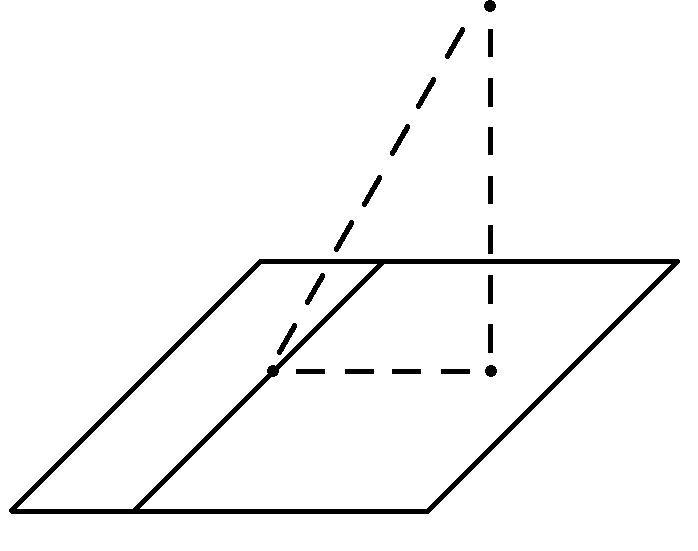
\includegraphics[width=\linewidth, height=2.0cm, right]{projection_hyp}
			\captionsetup{labelformat=empty}
			\put(-27, 60){$Y$}
			\put(-56, 41){\large $\searrow$}
			\put(-66, 53){$P_{H_0}$}
			\put(-46, 8){$P_1$}
			\put(-24, 38){$P_0$}
			\put(-98, 20){$L_{H_0}$}
			\put(-79, 11){\large $\searrow$}
			\put(-21, 5){$R(X)$}
		\end{minipage}
		\begin{minipage}{0.7\textwidth}
			\[H_0: K^Tb = 0 \quad \text{против} \quad H_1:K^Tb \neq 0, \]
			где $R(K) \subset R(X^T)$. В таком случае решающей величиной будет расстояние от $Y$ до пространства гипотезы:
			\[ L_{H_0} = \{ XB\ |\ K^Tb=0,\ b \in \MR^k \} \subset R(X). \]
		\end{minipage}
	\end{center}	
	Ортогональная проекция $Y$ на $L_{H_0}$: 
	\[P_{H_0} = P_0 - P_1,\]
	где
	\[ P_0 = X(X^TX)^-X^T \]
	и
	\[ P_1 = X(X^TX)^-K (K^T(X^TX)^-K)^- K^T(X^TX)^-X^T. \]
	$P_1$ также является ортогональное проекцией. При построении критерия разумно опираться на расстояние между $P_0Y$ и $P_{H_0}Y$. По теореме Пифагора:
	\[ \| (\mathbb{I}_n-P_{H_0})Y \|_2^2 - \| (\mathbb{I}_n-P_0)Y \|_2^2 =  \|P_1Y \|_2^2 = Y^TP_1Y. \]
	Последнее равенство следует из свойства идемпотентности матрицы $P_1$.
\end{rmrk}

\begin{thm}
	Пусть $Y \sim \mathcal{N}(\mu,\sigma^2 \mathbb{I}_n)$ и $P \in \MR^{n \times n}$, где $P^T=P$. Тогда $P$ -- ортогональная проекция тогда и только тогда, когда
	\[ Q = \frac{(Y - \mu)^T P (Y - \mu)}{\sigma^2} \sim \mathcal{X}_{r(P)}^2. \]
\end{thm}
\begin{proof} \\
	
	''$\Longrightarrow$'' Если $P^2 = P$, то существует $A \in \MR^{n \times n}$, где $A^TA = AA^T = \mathbb{I}_n$, такая что
	\[ A^TPA = \begin{pmatrix}
	\mathbb{I}_n & 0 \\
	0 & 0
	\end{pmatrix}, \]
	где $r = r(P)$. Мы знаем, что $Z = A^T(Y-\mu) \sim \mathcal{N}(0, \sigma^2 \mathbb{I}_n)$. Тогда
	\[ Q = \frac{(Y-\mu)^TP(Y-\mu)}{\sigma^2} = \frac{Z^TA^TPAZ}{\sigma^2} = \sum_{i=1}^{r}\Big( \frac{Z_i}{\sigma} \Big)^2 \sim \mathcal{X}_r^2.   \]
	
	''$\Longleftarrow$'' Так как $P^T=P$, существует матрица $B$, такая что $B^TB=BB^T=\mathbb{I}_n$ и
	\[ B^TPB = \Lambda = \diag(\lambda_1, \dots, \lambda_n),  \]
	где $\lambda_i$ -- вещественнозначные собственные числа $P$. Подставляя $X = B^T(Y-\mu) \sim \mathcal{N}(0, \sigma^2 \mathbb{I}_n )$, получаем
	\[ Q = \frac{1}{\sigma^2} X^TB^TPBX. \]
	Так как $Q \sim \mathcal{X}_r^2$, то её характеристическая функция:
	\[ \ME[\exp\{itQ\}] = (1-2it)^{-r/2}, \]
	и также:
	\[ \begin{aligned}
	\ME[\exp\{itQ\}] & = \ME \Big[ \exp\Big\{ \frac{it}{\sigma^2} X^TB^TPBX \Big\}\Big] = \ME \Big[ \exp\Big\{ it \sum_{j=1}^n \lambda_j \Big( \frac{X_j}{\sigma} \Big)^2 \Big\}\Big] \\
	& = \prod_{j=1}^{n} \ME \Big[ \exp\Big\{it \lambda_j \Big( \frac{X_j}{\sigma} \Big)^2 \Big \}\Big] = \prod_{j=1}^{n} (1 - 2it\lambda_j).
	\end{aligned} \]
	Поскольку полином однозначно определяется его линейными множителями, $\lambda_1 = \dots = \lambda_r = 1$ и $\lambda_j = 0 \ \forall j > r$. В частности,
	\[ P^2 = B\Lambda B^T B\Lambda B^T = B^T \Lambda^2 B^T= B\Lambda B^T = P. \]
\end{proof}

\begin{rmrk} \label{rmrk8.25}
	Пусть $Y \sim \mathcal{N}(\mu,\sigma^2 \mathbb{I}_n)$ и $P$ -- ортогональная проекция, где $r(P) = r$. Задав
	\[ A^TPA = \begin{pmatrix}
	\mathds{1}_r & 0 \\
	0 & 0
	\end{pmatrix},  \]
	мы получаем
	\[\widetilde{Q} = \frac{Y^TPY}{\sigma^2} = \frac{\widetilde{Z}^TA^TPA\widetilde{Z}}{\sigma^2},\]
	где
	\[ \widetilde{Z} = A^TY \sim \mathcal{N}(A^T\mu, \sigma^2\mathds{1}_n). \]
	Можно показать, что распределение
	\[ \widetilde{Q} = \sum_{i=1}^r \Big( \frac{\widetilde{Z}_i}{\sigma} \Big)^2  \]
	зависит только от $r$ и
	\[ \delta^2 = \sum_{i=1}^r \Big( \frac{(A^T\mu)_i}{\sigma} \Big)^2 = \frac{\mu^T P \mu}{\sigma^2}. \]
	Оно называется смещенным распределением $\mathcal{X}^2$ с $r$ степенями свободы и смещением $\delta^2$. Обозначение: $\widetilde{Q} \sim \mathcal{X}_{r, \delta^2}^2$.
\end{rmrk}

\begin{defn}
	Пусть $X \sim \mathcal{X}_m^2$ и $Y \sim \mathcal{X}_n^2$ независимы. 
	\begin{enumerate}
		\item Распределение случайной величины
		\[ F = \frac{nX}{mY} \]
		называется \textbf{\textit{F-распределением с $m$ и $n$ степенями свободы}}. Обозначение $F \sim F_{m,n}$.
		\item Если $X \sim \mathcal{X}_{m, \sigma^2}^2$, то
		\[ F = \frac{nX}{mY} \sim F_{m,n,\sigma^2}. \]
	\end{enumerate}
\end{defn}

\begin{thm}[\textbf{F-критерий в LMN}]
	В LMN пусть $R(K) \subset R(X^T)$, $t = r(K)$ и $r = r(X)$. Тогда
	\begin{enumerate}
		\item  \[ F = \frac{\frac{1}{t}\|P_1Y \|_2^2}{\frac{1}{n-r}\| RY \|_2^2} \sim F_{t, n-r, \delta^2}, \]
		где 
		\[\delta^2 = \frac{1}{\sigma^2} (K^Tb)^T(K^T(X^TX)^-K)^-K^Tb \]
	    и
	    \[ R = \mathbb{I} - P_0 \]
	    как прежде.
	    \item
	    \[ \varphi(Y) =
	    \left \{
	    \begin{array}{cl}
	    1, &  F >  F_{t, n-r, 1-\alpha}\\
	    0, & \text{иначе}. 
	    \end{array}
	    \right.
	    \]
	    -- \textbf{\textit{F-критерий}} для
	    \[ H_0: K^Tb = 0 \quad \text{против} \quad H_1: K^Tb \neq 0  \]
	    с уровнем значимости $\alpha$.
	\end{enumerate}
\end{thm}
\begin{proof}
	Достаточно показать (i). Из Замечания \ref{rmrk8.25} следует:
	\[ \frac{\| P_1Y \|_2^2}{\sigma^2} = \frac{Y^TP_1Y}{\sigma^2} \sim \mathcal{X}_{t, \delta^2}^2 \]
	и
	\[ \delta^2 = \frac{(Xb)^TP_1Xb}{\sigma^2} = \frac{(K^Tb)^T (K^T(X^TX)^-K)^-K^Tb}{\sigma^2}, \]
	исходя из определения $P_1$. Аналогично $\frac{Y^TRY}{\sigma^2} \sim \mathcal{X}_{n-r}$, так как $RXb = 0$. Лемма \ref{lmm8.15} и $P_1R=0$ завершают доказательство.
\end{proof}